\newpage
\begin{center}
    \section{S.M.O.I, une entreprise dans le secteur du bâtiment}
\end{center}

\subsection{Information général}
%\textbf{- coordonnée forme juridique et appartenance à un groupe, explication du gérant(qui et création de l'entreprise, choix de celle-ci)}

La société SMOI, d'un capital de 850000 euros, est installée sur l'île de la Réunion aux 120 route des sable - local 5 zone industriel des sable - 97427 l'Etang-Salé France, et est une SARL, créer le 2 Novembre 2016 à la suite de la cloturation d'établissements secondaires (d'abord le 1 Octobre 2005 puis le 02 Novembre 2016). Cette entreprise se situe dans le secteur du bâtiment comme principal activité la construction de charpentes métalliques. Elle fait partie du groupe Solution BTP O.I.\footnote{Groupe d'entreprise situé dans le secteur du bâtiment, fondé par M. VELETCHY le 6 Mars 2023 sous le nom SMOI-XL location et comprenant les entreprise SMOI, AMOI, TMOI, XL location, entreprise VELETCHY \& FRERES} \newline
Les locaux sont composé de deux partie, la partie atelier (où sont fabriquer les charpente) et la partie bureau (où sont organiser les réunion d'information sur le projet et dessiner les plans).\newline

Le gérant actuel de cette société est M.VELETCHY. Il est également le dirigeant de plusieurs autres entreprises étant dans des secteurs d'activités proches tel que le prêt de matériels de chantier, de véhicule de chantier, de transport de marchandise etc.



\subsection{SMOI aujourd'hui, qui en sont les principaux acteurs ?}
%\textbf{- organisation général de l'entreprise (service de l'atelier, dessin, RH, compta) Nombre de salariés et qualification, organisation du travail, production, fournisseur, clientèle, concurrence}

Cette entreprise est organisée en deux parties comme dit précédemment, la partie atelier et la partie bureau ou l'on retrouve plusieurs services avec un service dédié à la réalisation des plans des différents projets en fonction du cahier des charges, un service ressource humaine et un service comptabilité.\newline
Elle est spécialisée dans la construction de charpente métallique mais aussi de gros œuvre\footnote{cf lexique p14}. Ayant pour principaux fournisseurs Micab, Kdi Davum et Ravate pro( tous trois fournisseurs de matériaux de construction et équipement). Et étant en concurrence directe avec de nombreuses autres entreprises tel que GTOI\footnote{Les grands travaux de l'océan Indien}, ou encore SARL Freres Lebon...\newline
Cette entreprise de 25 salariés vise principalement des particuliers avec par exemple la création d'une passerelle pour un cabinet de médecin, mais celle-ci intervient également sur de plus gros chantiers.



\subsection{Les politique d'hygiène et de sécurité dans l'entreprise}
%\textbf{- parler du qcm et faire ref à l'annexe}

Cette entreprise étant accès sur la construction de charpente métallique, présente de nombreux risque au niveau de la sécurité de ses salariés, il y a alors des politique qui sont mis en place ainsi qu'un certain nombre de réglementation à respecter afin de pouvoir entrer dans l'atelier (port obligatoire de protection visuelle, auditive, gants, tenu de travaille ininflammable, chaussure de chantier et casque de protection), des politiques et nouvelle norme de sécurité sont régulièrement mis en place, lors de réunion annuelle (avec la modification du Document Unique) visant à ré-évaluer les risque encouru par les employés lors des mission qui leur sont attribués, en fonction du nouveau matériel à acquérir ou non mais aussi en fonction des nouvelle tâche demandée dont les risque pourrait ne pas encore figurer dans le document et dont les mesure de sécurité ne serait alors pas encore prescrite.\newline
Un moyen de prévention cependant trop peu contrôlé, en effet il n'y a aucun suivi de la bonne réalisation et suivit de ce programme d'action mis en place ni de CSE\footnote{Comité sociale économique, l'anciennement Comité Hygiène et Sécurité des conditions de travail}. Il y a cependant des vérification régulière qui sont faite sur le matériel tel que les véhicule de chantier ou filet de protection.\footnote{cf annexe 1}



\subsection{SMOI, une entreprise engagé dans un esprit socio-écologique}
%\textbf{- parler du qcm et faire ref à l'annexe}

Malgré le fait que SMOI ne possède pas de service lié aux enjeux socio-écologique, celle-ci met en place des mesure afin de réduire son empreinte écologique et de préserver l'environnement, avec la présence d'un tri des matière première usé lors de la fabrication ainsi qu'un projet de mise en place d'une fosse hydrocarbure pour récupérer l'huile utilisé. Une partie de cet engagement se retrouve également dans une politique d'hygiène mise en place, qui est le nettoyage de l'atelier tous les vendredi soir, faisant le tri des métaux usés et un nettoyage méticuleux des sols tout en essayant au maximum de préserver l'environnement par ces actions. \newline

SMOI fait également appel à d'autres prestataires extérieurs afin de pouvoir faire le point sur ces conditions écologiques et enjeux importants et de mettre en place des solutions et méthodes. Et malgré l'absence de politique de réduction des émissions de gaz à effet de serre, il y a la présence de réunions chaque trimestre visant à faire le point cette fois-ci en interne sur les politique réaliser, la suivi de ces actions et une réflexion sur la possible mise en place d'autres.\footnote{cf annexe 3}



\subsection{Une entreprise qui cependant a de nombreuse difficultés}
%\textbf{- finance, plan de redressement}

La société SMOI est cependant depuis 2016 en difficulté financière avec une baisse de son chiffre d'affaires passant de 7.35M en 2016 à 2.38M en 2022 comme le montre ce graphique ci-dessous \ref{fig:CA_SMOI}.
\begin{figure}[h!]
    \centering
    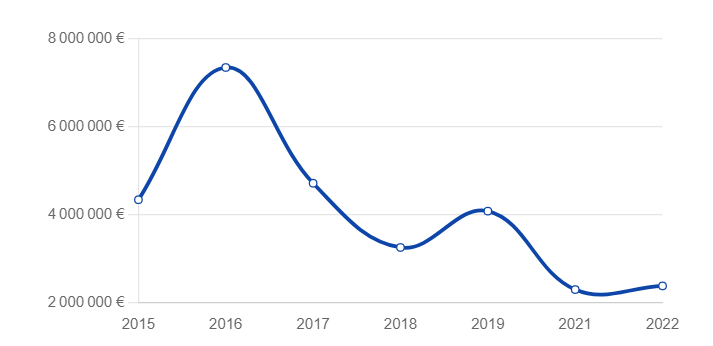
\includegraphics[width=0.75\textwidth]{figures/CA_SMOI.png}
    \caption{Évolution du chiffre d'affaire de la société SMOI de 2015 à 2022}
    \label{fig:CA_SMOI}
\end{figure}\newpage
Des difficultés se ressentent dans la quasi-totalité des entreprises du groupe \textit{Solution BTP O.I.} visible par l'évolution des résultats net du groupe. \ref{fig:résultat_solBTP}
\begin{figure}[h!]
    \centering
    \includegraphics[width=0.75\linewidth]{figures/résultat_solBTP.png}
    \caption{Évolution des résultats net du groupe Solution BTP O.I.}
    \label{fig:résultat_solBTP}
\end{figure}\newline
Il a donc été pris comme décision en Juillet/Août 2023 (donc durant ma période de stage) de dissoudre les société du groupe \textit{Solution BTP O.I.} et de transmettre leur capital social à l'entreprise \textit{Solution BTP O.I.} et ainsi de provoquer la fusion de toutes les entreprises en une seule afin de réduire les charges appliquées à celles-ci et permettre de relancer l'activité. En effet, depuis le 10 février 2022 et jusqu'au 21 Mars 2023 la société SMOI avait demander un plan de redressement judiciaire afin de pouvoir permettre d'avoir le temps de relancer l'activité, une procédure qui aboutira sur la fusion, cité précédemment, des entreprises du groupe en une \textit{Solution BTP O.I.} de nom commercial: \textsc{SMOI-XL location}.\footnote{cf annexe 4}\newline



\subsection{AMOI, l'atelier de SMOI.}
%\textbf{- moi dans l'entreprise, organigramme + technologie}

Cette entreprise, notamment sa partie atelier, \acrshort{AMOI}* qui grâce à sa proximité avec d'autre entreprise de prêt de matériel et véhicule de chantier, à accès à ceux-ci tel que des chariot élévateur et/ou des grues ainsi que des technologie de découpe plasma, des machine de pliage et de découpe de tôle et d'autre matière première métallique.\newline
J'ai réalisé mon stage dans ce secteur de l'entreprise chargée de la construction des charpentes suivant les plans réalisés par SMOI. Un atelier composé d'un responsable ayant les diplômes pour exercer et gérer les métiers dans l'atelier, de trois ouvriers de chantier, d'un chargé de la quincaillerie, et d'un chargé de la peinture et du revêtement des charpentes, organisé comme ci-contre dans cette organigramme.\ref{fig:organigram_AMOI}
\begin{figure}[h!]
    \centering
    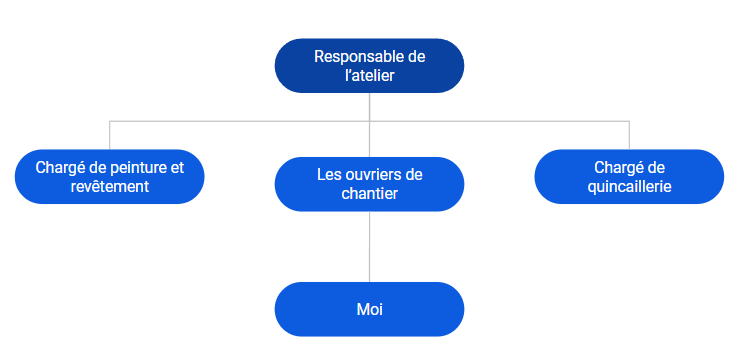
\includegraphics[width=1\linewidth]{figures/organigram_AMOI.png}
    \caption{Organigramme de AMOI}
    \label{fig:organigram_AMOI}
\end{figure} \newline


\subsubsection{Conclusion}
%résumer des information importante de cette première partie

Pour conclure cette partie, j'ai réalisé mon stage dans l'atelier de construction métallique de la société SMOI, une entreprise du secteur du bâtiment, qui faisait partie du groupe \textit{Solution BTP O.I.} et qui aujourd'hui est devenue la société \textit{SMOI-XL location} suite à un plan de redressement et la fusion de toutes les entreprises du groupe \textit{Solution BTP O.I.}. De plus, j'ai pu constater que cette entreprise avait des normes de sécurité et revue régulièrement en prenant en compte les missions données et qu'elle prenait également en compte les enjeux socio-écologiques actuels dans son fonctionnement.
